
%% bare_conf.tex
%% V1.3
%% 2007/01/11
%% by Michael Shell
%% See:
%% http://www.michaelshell.org/
%% for current contact information.
%%
%% This is a skeleton file demonstrating the use of IEEEtran.cls
%% (requires IEEEtran.cls version 1.7 or later) with an IEEE conference paper.
%%
%% Support sites:
%% http://www.michaelshell.org/tex/ieeetran/
%% http://www.ctan.org/tex-archive/macros/latex/contrib/IEEEtran/
%% and
%% http://www.ieee.org/

%%*************************************************************************
%% Legal Notice:
%% This code is offered as-is without any warranty either expressed or
%% implied; without even the implied warranty of MERCHANTABILITY or
%% FITNESS FOR A PARTICULAR PURPOSE!
%% User assumes all risk.
%% In no event shall IEEE or any contributor to this code be liable for
%% any damages or losses, including, but not limited to, incidental,
%% consequential, or any other damages, resulting from the use or misuse
%% of any information contained here.
%%
%% All comments are the opinions of their respective authors and are not
%% necessarily endorsed by the IEEE.
%%
%% This work is distributed under the LaTeX Project Public License (LPPL)
%% ( http://www.latex-project.org/ ) version 1.3, and may be freely used,
%% distributed and modified. A copy of the LPPL, version 1.3, is included
%% in the base LaTeX documentation of all distributions of LaTeX released
%% 2003/12/01 or later.
%% Retain all contribution notices and credits.
%% ** Modified files should be clearly indicated as such, including  **
%% ** renaming them and changing author support contact information. **
%%
%% File list of work: IEEEtran.cls, IEEEtran_HOWTO.pdf, bare_adv.tex,
%%                    bare_conf.tex, bare_jrnl.tex, bare_jrnl_compsoc.tex
%%*************************************************************************

% *** Authors should verify (and, if needed, correct) their LaTeX system  ***
% *** with the testflow diagnostic prior to trusting their LaTeX platform ***
% *** with production work. IEEE's font choices can trigger bugs that do  ***
% *** not appear when using other class files.                            ***
% The testflow support page is at:
% http://www.michaelshell.org/tex/testflow/



% Note that the a4paper option is mainly intended so that authors in
% countries using A4 can easily print to A4 and see how their papers will
% look in print - the typesetting of the document will not typically be
% affected with changes in paper size (but the bottom and side margins will).
% Use the testflow package mentioned above to verify correct handling of
% both paper sizes by the user's LaTeX system.
%
% Also note that the "draftcls" or "draftclsnofoot", not "draft", option
% should be used if it is desired that the figures are to be displayed in
% draft mode.
%
\documentclass[conference]{IEEEtran}
% Add the compsoc option for Computer Society conferences.
%
% If IEEEtran.cls has not been installed into the LaTeX system files,
% manually specify the path to it like:
% \documentclass[conference]{../sty/IEEEtran}





% Some very useful LaTeX packages include:
% (uncomment the ones you want to load)


% *** MISC UTILITY PACKAGES ***
%
%\usepackage{ifpdf}
% Heiko Oberdiek's ifpdf.sty is very useful if you need conditional
% compilation based on whether the output is pdf or dvi.
% usage:
% \ifpdf
%   % pdf code
% \else
%   % dvi code
% \fi
% The latest version of ifpdf.sty can be obtained from:
% http://www.ctan.org/tex-archive/macros/latex/contrib/oberdiek/
% Also, note that IEEEtran.cls V1.7 and later provides a builtin
% \ifCLASSINFOpdf conditional that works the same way.
% When switching from latex to pdflatex and vice-versa, the compiler may
% have to be run twice to clear warning/error messages.






% *** CITATION PACKAGES ***
%
%\usepackage{cite}
% cite.sty was written by Donald Arseneau
% V1.6 and later of IEEEtran pre-defines the format of the cite.sty package
% \cite{} output to follow that of IEEE. Loading the cite package will
% result in citation numbers being automatically sorted and properly
% "compressed/ranged". e.g., [1], [9], [2], [7], [5], [6] without using
% cite.sty will become [1], [2], [5]--[7], [9] using cite.sty. cite.sty's
% \cite will automatically add leading space, if needed. Use cite.sty's
% noadjust option (cite.sty V3.8 and later) if you want to turn this off.
% cite.sty is already installed on most LaTeX systems. Be sure and use
% version 4.0 (2003-05-27) and later if using hyperref.sty. cite.sty does
% not currently provide for hyperlinked citations.
% The latest version can be obtained at:
% http://www.ctan.org/tex-archive/macros/latex/contrib/cite/
% The documentation is contained in the cite.sty file itself.






% *** GRAPHICS RELATED PACKAGES ***
%
\ifCLASSINFOpdf
  % \usepackage[pdftex]{graphicx}
  % declare the path(s) where your graphic files are
  % \graphicspath{{../pdf/}{../jpeg/}}
  % and their extensions so you won't have to specify these with
  % every instance of \includegraphics
  % \DeclareGraphicsExtensions{.pdf,.jpeg,.png}
\else
  % or other class option (dvipsone, dvipdf, if not using dvips). graphicx
  % will default to the driver specified in the system graphics.cfg if no
  % driver is specified.
  % \usepackage[dvips]{graphicx}
  % declare the path(s) where your graphic files are
  % \graphicspath{{../eps/}}
  % and their extensions so you won't have to specify these with
  % every instance of \includegraphics
  % \DeclareGraphicsExtensions{.eps}
\fi
% graphicx was written by David Carlisle and Sebastian Rahtz. It is
% required if you want graphics, photos, etc. graphicx.sty is already
% installed on most LaTeX systems. The latest version and documentation can
% be obtained at:
% http://www.ctan.org/tex-archive/macros/latex/required/graphics/
% Another good source of documentation is "Using Imported Graphics in
% LaTeX2e" by Keith Reckdahl which can be found as epslatex.ps or
% epslatex.pdf at: http://www.ctan.org/tex-archive/info/
%
% latex, and pdflatex in dvi mode, support graphics in encapsulated
% postscript (.eps) format. pdflatex in pdf mode supports graphics
% in .pdf, .jpeg, .png and .mps (metapost) formats. Users should ensure
% that all non-photo figures use a vector format (.eps, .pdf, .mps) and
% not a bitmapped formats (.jpeg, .png). IEEE frowns on bitmapped formats
% which can result in "jaggedy"/blurry rendering of lines and letters as
% well as large increases in file sizes.
%
% You can find documentation about the pdfTeX application at:
% http://www.tug.org/applications/pdftex





% *** MATH PACKAGES ***
%
%\usepackage[cmex10]{amsmath}
% A popular package from the American Mathematical Society that provides
% many useful and powerful commands for dealing with mathematics. If using
% it, be sure to load this package with the cmex10 option to ensure that
% only type 1 fonts will utilized at all point sizes. Without this option,
% it is possible that some math symbols, particularly those within
% footnotes, will be rendered in bitmap form which will result in a
% document that can not be IEEE Xplore compliant!
%
% Also, note that the amsmath package sets \interdisplaylinepenalty to 10000
% thus preventing page breaks from occurring within multiline equations. Use:
%\interdisplaylinepenalty=2500
% after loading amsmath to restore such page breaks as IEEEtran.cls normally
% does. amsmath.sty is already installed on most LaTeX systems. The latest
% version and documentation can be obtained at:
% http://www.ctan.org/tex-archive/macros/latex/required/amslatex/math/





% *** SPECIALIZED LIST PACKAGES ***
%
%\usepackage{algorithmic}
% algorithmic.sty was written by Peter Williams and Rogerio Brito.
% This package provides an algorithmic environment fo describing algorithms.
% You can use the algorithmic environment in-text or within a figure
% environment to provide for a floating algorithm. Do NOT use the algorithm
% floating environment provided by algorithm.sty (by the same authors) or
% algorithm2e.sty (by Christophe Fiorio) as IEEE does not use dedicated
% algorithm float types and packages that provide these will not provide
% correct IEEE style captions. The latest version and documentation of
% algorithmic.sty can be obtained at:
% http://www.ctan.org/tex-archive/macros/latex/contrib/algorithms/
% There is also a support site at:
% http://algorithms.berlios.de/index.html
% Also of interest may be the (relatively newer and more customizable)
% algorithmicx.sty package by Szasz Janos:
% http://www.ctan.org/tex-archive/macros/latex/contrib/algorithmicx/




% *** ALIGNMENT PACKAGES ***
%
%\usepackage{array}
% Frank Mittelbach's and David Carlisle's array.sty patches and improves
% the standard LaTeX2e array and tabular environments to provide better
% appearance and additional user controls. As the default LaTeX2e table
% generation code is lacking to the point of almost being broken with
% respect to the quality of the end results, all users are strongly
% advised to use an enhanced (at the very least that provided by array.sty)
% set of table tools. array.sty is already installed on most systems. The
% latest version and documentation can be obtained at:
% http://www.ctan.org/tex-archive/macros/latex/required/tools/


%\usepackage{mdwmath}
%\usepackage{mdwtab}
% Also highly recommended is Mark Wooding's extremely powerful MDW tools,
% especially mdwmath.sty and mdwtab.sty which are used to format equations
% and tables, respectively. The MDWtools set is already installed on most
% LaTeX systems. The lastest version and documentation is available at:
% http://www.ctan.org/tex-archive/macros/latex/contrib/mdwtools/


% IEEEtran contains the IEEEeqnarray family of commands that can be used to
% generate multiline equations as well as matrices, tables, etc., of high
% quality.


%\usepackage{eqparbox}
% Also of notable interest is Scott Pakin's eqparbox package for creating
% (automatically sized) equal width boxes - aka "natural width parboxes".
% Available at:
% http://www.ctan.org/tex-archive/macros/latex/contrib/eqparbox/





% *** SUBFIGURE PACKAGES ***
%\usepackage[tight,footnotesize]{subfigure}
% subfigure.sty was written by Steven Douglas Cochran. This package makes it
% easy to put subfigures in your figures. e.g., "Figure 1a and 1b". For IEEE
% work, it is a good idea to load it with the tight package option to reduce
% the amount of white space around the subfigures. subfigure.sty is already
% installed on most LaTeX systems. The latest version and documentation can
% be obtained at:
% http://www.ctan.org/tex-archive/obsolete/macros/latex/contrib/subfigure/
% subfigure.sty has been superceeded by subfig.sty.



%\usepackage[caption=false]{caption}
%\usepackage[font=footnotesize]{subfig}
% subfig.sty, also written by Steven Douglas Cochran, is the modern
% replacement for subfigure.sty. However, subfig.sty requires and
% automatically loads Axel Sommerfeldt's caption.sty which will override
% IEEEtran.cls handling of captions and this will result in nonIEEE style
% figure/table captions. To prevent this problem, be sure and preload
% caption.sty with its "caption=false" package option. This is will preserve
% IEEEtran.cls handing of captions. Version 1.3 (2005/06/28) and later
% (recommended due to many improvements over 1.2) of subfig.sty supports
% the caption=false option directly:
%\usepackage[caption=false,font=footnotesize]{subfig}
%
% The latest version and documentation can be obtained at:
% http://www.ctan.org/tex-archive/macros/latex/contrib/subfig/
% The latest version and documentation of caption.sty can be obtained at:
% http://www.ctan.org/tex-archive/macros/latex/contrib/caption/




% *** FLOAT PACKAGES ***
%
%\usepackage{fixltx2e}
% fixltx2e, the successor to the earlier fix2col.sty, was written by
% Frank Mittelbach and David Carlisle. This package corrects a few problems
% in the LaTeX2e kernel, the most notable of which is that in current
% LaTeX2e releases, the ordering of single and double column floats is not
% guaranteed to be preserved. Thus, an unpatched LaTeX2e can allow a
% single column figure to be placed prior to an earlier double column
% figure. The latest version and documentation can be found at:
% http://www.ctan.org/tex-archive/macros/latex/base/



%\usepackage{stfloats}
% stfloats.sty was written by Sigitas Tolusis. This package gives LaTeX2e
% the ability to do double column floats at the bottom of the page as well
% as the top. (e.g., "\begin{figure*}[!b]" is not normally possible in
% LaTeX2e). It also provides a command:
%\fnbelowfloat
% to enable the placement of footnotes below bottom floats (the standard
% LaTeX2e kernel puts them above bottom floats). This is an invasive package
% which rewrites many portions of the LaTeX2e float routines. It may not work
% with other packages that modify the LaTeX2e float routines. The latest
% version and documentation can be obtained at:
% http://www.ctan.org/tex-archive/macros/latex/contrib/sttools/
% Documentation is contained in the stfloats.sty comments as well as in the
% presfull.pdf file. Do not use the stfloats baselinefloat ability as IEEE
% does not allow \baselineskip to stretch. Authors submitting work to the
% IEEE should note that IEEE rarely uses double column equations and
% that authors should try to avoid such use. Do not be tempted to use the
% cuted.sty or midfloat.sty packages (also by Sigitas Tolusis) as IEEE does
% not format its papers in such ways.





% *** PDF, URL AND HYPERLINK PACKAGES ***
%
%\usepackage{url}
% url.sty was written by Donald Arseneau. It provides better support for
% handling and breaking URLs. url.sty is already installed on most LaTeX
% systems. The latest version can be obtained at:
% http://www.ctan.org/tex-archive/macros/latex/contrib/misc/
% Read the url.sty source comments for usage information. Basically,
% \url{my_url_here}.





% *** Do not adjust lengths that control margins, column widths, etc. ***
% *** Do not use packages that alter fonts (such as pslatex).         ***
% There should be no need to do such things with IEEEtran.cls V1.6 and later.
% (Unless specifically asked to do so by the journal or conference you plan
% to submit to, of course. )

\usepackage{url}
\usepackage{subfig}
\usepackage{graphicx}
\usepackage{epstopdf}
\usepackage{flushend}
\usepackage{listings}
\usepackage{color}
\usepackage{multicol}
\usepackage{amsmath}

\newtheorem{definition}{Definition}

% correct bad hyphenation here
\hyphenation{op-tical net-works semi-conduc-tor}



\definecolor{dkgreen}{rgb}{0,0.6,0}
\definecolor{gray}{rgb}{0.5,0.5,0.5}
\definecolor{mauve}{rgb}{0.58,0,0.82}

\lstset{
  language=Java,
  aboveskip=3mm,
  belowskip=3mm,
  showstringspaces=false,
  columns=flexible,
  basicstyle={\footnotesize\ttfamily},
  numbers=none,
  numberstyle=\tiny\color{gray},
  keywordstyle=\color{blue},
  commentstyle=\color{dkgreen},
  stringstyle=\color{mauve},
  breaklines=true,
  breakatwhitespace=true
  tabsize=3
}


\begin{document}
%
% paper title
% can use linebreaks \\ within to get better formatting as desired
\title{Framework for Collection of Electrophysiology Data Across Heterogeneous Databases}


% author names and affiliations
% use a multiple column layout for up to three different
% affiliations
\author{\IEEEauthorblockN{Petr Je\v{z}ek, Roman Mou\v{c}ek}
\IEEEauthorblockN{Jakub Krauz, Jaroslav Ho\v{s}ek}
\IEEEauthorblockA{Department of Computer Science\\ and Engineering\\
New Technologies for the Information Society\\
Faculty of Applied Sciences\\
University of West Bohemia\\
Plzen, Czech Republic\\
{jezekp, moucek, krauz, axim}@kiv.zcu.cz}
\and
\IEEEauthorblockN{Yann Le Franc}
\IEEEauthorblockA{Theoretical Neurobiology\\ and Neuroengineering lab\\
Department Biomedical Science\\
University of Antwerp\\
Wilrijk, Belgium\\
$\&$ e-Neuroscience Consulting Network\\
ylefranc@gmail.com}
\and
\IEEEauthorblockN{Thomas Wachtler, Jan Grewe}
\IEEEauthorblockA{Department Biologie II\\
Ludwig-Maximilians-Universit\"at M\"unchen\\
 Planegg-Martinsried, Germany\\
{wachtler, grewe}@biologie.uni-munchen.de}}

% conference papers do not typically use \thanks and this command
% is locked out in conference mode. If really needed, such as for
% the acknowledgment of grants, issue a \IEEEoverridecommandlockouts
% after \documentclass

% for over three affiliations, or if they all won't fit within the width
% of the page, use this alternative format:
%
%\author{\IEEEauthorblockN{Michael Shell\IEEEauthorrefmark{1},
%Homer Simpson\IEEEauthorrefmark{2},
%James Kirk\IEEEauthorrefmark{3},
%Montgomery Scott\IEEEauthorrefmark{3} and
%Eldon Tyrell\IEEEauthorrefmark{4}}
%\IEEEauthorblockA{\IEEEauthorrefmark{1}School of Electrical and Computer Engineering\\
%Georgia Institute of Technology,
%Atlanta, Georgia 30332--0250\\ Email: see http://www.michaelshell.org/contact.html}
%\IEEEauthorblockA{\IEEEauthorrefmark{2}Twentieth Century Fox, Springfield, USA\\
%Email: homer@thesimpsons.com}
%\IEEEauthorblockA{\IEEEauthorrefmark{3}Starfleet Academy, San Francisco, California 96678-2391\\
%Telephone: (800) 555--1212, Fax: (888) 555--1212}
%\IEEEauthorblockA{\IEEEauthorrefmark{4}Tyrell Inc., 123 Replicant Street, Los Angeles, California 90210--4321}}




% use for special paper notices
%\IEEEspecialpapernotice{(Invited Paper)}




% make the title area
\maketitle


\begin{abstract}
%\boldmath
Experiments in electrophysiology produce a lot of unstructured metadata collected in electrophysiology databases. The data are usually accessed through a web interface implemented on the top of data model respecting given data format. A lot of experiments are conducted outside the laboratory where access to these databases is not always available. The usage of mobile devices such as tablets or smart phones seems to be a practical solution, but users would welcome the same structured user interface such as they know from a common computer. When user interfaces of electrophysiology databases are tailored to a unique data structure, they cannot be easily reused on a mobile device. As a solution, a mapping of a general data structure to a graphical template is proposed. This mapping is implemented in a framework that generates a template representing the database structure. The parsing process is driven by supplemented annotations added to the code. Next, an Android tool visualizing a graphical layout generated from the template is developed. A use case study is presented on a database of EEG/ERP experiments.
\end{abstract}
% IEEEtran.cls defaults to using nonbold math in the Abstract.
% This preserves the distinction between vectors and scalars. However,
% if the conference you are submitting to favors bold math in the abstract,
% then you can use LaTeX's standard command \boldmath at the very start
% of the abstract to achieve this. Many IEEE journals/conferences frown on
% math in the abstract anyway.

% no keywords




% For peer review papers, you can put extra information on the cover
% page as needed:
% \ifCLASSOPTIONpeerreview
% \begin{center} \bfseries EDICS Category: 3-BBND \end{center}
% \fi
%
% For peerreview papers, this IEEEtran command inserts a page break and
% creates the second title. It will be ignored for other modes.
\IEEEpeerreviewmaketitle



\section{Introduction}\label{Introduction}

Large collections of data sets are obtained during electrophysiological experiments. With increasing number of experiments a crucial task is to provide metadata descriptions. These metadata usually include experimental constraints and scenarios, and information about tested subject. Raw data without descriptive metadata are meaningless. At present due to the penetration of computers into medicine collections of electrophysiology metadata are moved from paper forms to specialized electrophysiological databases. These databases are accessed via desktop or web based user interfaces using common computers. However, there are common situations when a classic computer is not available. These situations occur in environments such as hospitals or prisons where a wireless connection is usually unavailable. In addition, a lot of experiments are conducted outside laboratories using portable measuring devices. In this case data are obtained offline and then must be backward synchronized with data stored in an electrophysiological database. Electrophysiological databases are based on specific data model. User interfaces implemented on the top of these models are non-transferable to other data models. Development of various user interfaces is time consuming, and there are difficult to maintain, consequently it reduces users experience. As a solution we present an annotation based framework that aim is to generate a template for client applications. This template contains description of metadata structure of an electrophysiological database. A graphical layout for a specific device is then generated according to the obtained template.  As a first pilot system we have implemented an Android based system that generates a template for mobile devices such as tablets or cell-phones. These devices are connected to the electrophysiological database through the framework API.

The structure of the paper is following. First, we briefly introduce existing electrophysiological databases and mobile-based approaches. Then, we describe a proposed mapping that maps the data model of a database to a template expressed in a transport format. Next, we introduce an implementation of proposed mapping in the framework. The rest of the paper describes validation of the presented approach as a part of a use-case study in which integration of the framework in EEGBase \cite{ISI:000306821100004} is demonstrated.

\section{State of the Art}

Research in the electrophysiology domain faces a lack of tools and infrastructure for collecting and processing experimental data. There are several organizations implementing an providing tools for data processing, electrophysiological databases or hardware devices. Lots of them are the members of international neuroinformatics community that activities are led by International Neuroinformatics Coordinating Facility (INCF)\footnote{http://www.incf.org/}.

CRCNS \cite{CRCNS} provides marketplace and discussion forum for sharing tools and data in neuroscience. Helmholtz \cite{10.3389/conf.fninf.2013.09.00025} is a framework for creating neuroscience databases that are customized to the needs of individual neurophysiology labs. G-Node \cite{GNODE2013} provides tools for data access, data management and data sharing. Carmen \cite{fgibson:Watson2007} is a virtual laboratory that enables a storage of experimental data, experimental protocols, or analysis code; it designs workflows from the stored code and run them remotely. EEGBase is a database of well-described EEG/ERP experimental data sets that enables users to upload, download and manage own experiments, INCF Dataspace \cite{dataspace} enables interested research groups to connect to a distributed data file system based on iRods\footnote{http://irods.org/}.

The described solutions provide robust and flexible databases and tools in environments where a common computer is available. When a researcher is working out of laboratory, paper forms that are backwards transferred to a database, are usually used. Several initiatives and pilot studies remove this tedious and error prone work by developing portable devices as specialized laptops, mobile phones and tablets.


Clinician Assessment and Remote Administration Tablet (CARAT) \cite{10.3389/fninf.2011.00031} is a Microsoft Windows tablet adapted to collect and administer clinical assessments in large scale demographic or neuropsychiatric studies. It uses an architecture with two modules. The first one setups the clinical study while the second one serves to data collection. Collected data are synchronized with a remote database.

Research Electronic Data Capture \cite{journals/bmcbi/Harris12} (REDCap) is a software application and workflow methodology designed to collect and manage data for research studies. REDCap Mobile \cite{Borlawsky01122011} is a solution that describes encrypted laptops with a push-pull relationship to the centralized REDCap database to allow data collection while off-line.

A mobile EEGBase client \cite{10.3389/conf.fninf.2013.09.00046} enables users to collect data from EEG/ERP experiments and provides an online synchronization with EEGBase.

\section{Proposed Framework}\label{Framework}

\subsection{System Restrictions and Requirements}

Facing difficulties mentioned in Section \ref{Introduction} we decided to design and implement a tool that facilitates collection of metadata from experiments by a unified interface customizable to the data structure. In order to ensure an immediate usage, the user interface must be easily generated. In addition, the synchronization of collected data with the electrophysiology database is crucial in the perspective of their sharing and management.

Respecting the requirements from previous paragraph we defined several restrictions that the system must fulfill. It must be inherently client-server oriented. The server end must provide a well-known API to be integrated with most common electrophysiology databases. Moreover, the server and the client must communicate using a unified data format to be easily migrated across different platforms and to be understandable by various clients.

The client end parses the exported data structure and generates a graphical layout. Once the layout is generated, the user can customize it. When the user has the layout prepared, the client is able to download data from the server or push data stored locally. When the client works offline, the data must be stored in an embedded database and synchronized immediately when the client gets back online.

On the other hand, a lot of researchers do not have an access to an electrophysiology database. For such users there is a possibility to define a layout from an empty template without necessity to download the template from the server.

The idea initially presented in \cite{6645264} described a client-server system. The server is able to annotate the database layer of an electrophysiology database. Such annotated layer is then serialized to a XML structure and sent to the client. This idea is extended, implemented and validated in this paper.

\subsection{Mapping Annotated Code to Data Template}\label{Mapping_Code_To_Template}

Modern systems are coded using high-level virtual machine programming languages such as Java, .NET or Python. These languages rely on reflection an ability of a computer program to examine and modify the structure at runtime. Moreover, the code in these languages can be annotated by supplemented metadata. These metadata can be processed by reflection at runtime. Java uses Java Reflection API \cite{1932394184} to read Java Annotations \cite{AnnotationsJavaDevGuide}. These annotations give additional semantic meaning to common Java classes. When a database layer in Java programs is represented by POJOs\footnote{Plain Old Java Object - A Java class with class attributes accessed by get/set methods}, a suitable approach is their extension by specially designed annotations. These annotations provide the means to describe a data template.

As a solution we designed a set of annotations described in Table \ref{annotations}. The annotation \texttt{@Form} represents one form on the layout. If one form is represented by more than one entity, the annotation \texttt{@Multiform} with the same name is used for each entity included in the form. The \texttt{@FormItem} annotation denotes attributes that appear in a specific form. The \texttt{@FormItemRestriction} annotation defines restrictions on individual items. These restrictions can be e. g. minimal and maximal numerical values or maximal length of text values.

% Table generated by Excel2LaTeX from sheet 'List1'
\begin{table}
\begin{tabular}{|l|l|l|}
\hline
{\bf Annotation} & {\bf Parameter} & {\bf Meaning} \\
\hline
     @Form &      label & Label of the form. \\
\hline
@FormDescription &      value & The description. \\
\hline
\multicolumn{ 1}{|l|}{@MultiForm} &      value & Identifier of the form (string). \\

\multicolumn{ 1}{|l|}{} &      label & Label of the form. \\
\hline
\multicolumn{ 1}{|l|}{@FormItem} &      label & Label of the item. \\

\multicolumn{ 1}{|l|}{} &   required & Determines a required value (default: false) \\

\multicolumn{ 1}{|l|}{} &    preview & Determines items used in data previews. \\
\hline
\multicolumn{ 1}{|l|}{@FormItemRestriction} &  minLength & Minimum length of the input. \\

\multicolumn{ 1}{|l|}{} &  maxLength & Maximum length of the input. \\

\multicolumn{ 1}{|l|}{} &   minValue & Minimum value of numerical item. \\

\multicolumn{ 1}{|l|}{} &   maxValue & Maximum value of numerical item. \\

\multicolumn{ 1}{|l|}{} & defaultValue & The default value. \\

\multicolumn{ 1}{|l|}{} &     values & Enumeration of possible values. \\
\hline
\end{tabular}
\caption{\label{annotations}Supported Annotations}
\end{table}

When the data layer of the database is annotated, it must be mapped to a suitable transport format. Formats solve description of electrophysiology data on different levels of abstraction from low-level binary formats, through highly abstract implementation-independent data formats till formats based on semantic web ontologies. Each approach has its benefits and difficulties needed to be overcome. We require a format that provides a sufficient level of abstraction to be system independent on one hand, but it is easy-to-use without any specific requirements for user's knowledge on the other hand. The most flexible ones are Hierarchical Data Format (HDF5) \cite{hdf5} or respectively epHDF that is a specialized HDF5 for electrophysiology. HDF5 and epHDF5 are containers for raw binary data and metadata represented in the JSON\footnote{http://json.org/} format. The is odML \cite{10.3389/fninf.2011.00016} is an open format to store and transport metadata more then a container for data. This format brings the following advantages: (1) platform-independence, (2) simplicity and human-readability, (3) ability to transfer layouts as well as metadata with the same format. Because of mentioned benefits of odML we selected it for the framework.


\section{Implementation}


\subsection{Mapping Implementation}


The mapping presented in Section \ref{Mapping_Code_To_Template} shows transferring persistent Java classes to templates. Then, these templates are mapped to odML representation and transferred to the client. OdML is based on \textit{Sections} that can contain \textit{Properties} and \textit{Values}. Moreover, each section can contain subsections (tree-like structures can be created). Definition \ref{def:Java_annotation_extraction_process} formalizes an extraction process from Java Annotations to corresponding odML representation.

\begin{definition}
\label{def:Java_annotation_extraction_process}
(Java annotation extraction process)

\emph{The process is the transformation of a set of Java annotations JA to an odML Section S in the odML document D that satisfies:}

\emph{$\forall$ $JA{}_{\text{i}}\in {(@Form)}$ $\exists$ odML Section $S{}_{\text{i}}$ $\in$ D $\Rightarrow$ $JA{}_{\text{i}}$ $\in$ a class annotation}.

\emph{$\forall$ $JA{}_{\text{j}}\in {(@FormItem)}$ $\exists$ odML Section $S{}_{\text{j}}$ $\subset$ $S{}_{\text{i}}$ $\in$ D $\Rightarrow$ $JA{}_{\text{j}}$ $\in$ a property
annotation}.

\emph{$\forall$ $JA{}_{\text{k}}\in {(@FormRestriction)}$ $\exists$ odML Property $P{}_{\text{k}}$ $\in$ $S{}_{\text{j}}$ $\in$ D $\Rightarrow$ $JA{}_{\text{k}}$ $\in$ a property  annotation}.

\end{definition}

Listing \ref{class_ex} shows an Example of the class \textit{Person} containing several attributes \textit{givenname}, \textit{surname} and \textit{gender} supplemented by metadata annotations (other annotations, class imports, get/set methods, and other fields are omitted for simplicity).

A XML serialization of this class to an odML document is presented in Listing \ref{odml_rep}. The document shows one section named \textit{Person} with a subsection \textit{gender} (note: Because of XML serialization is quite long, similar subsections representing other attributes are omitted). All restrictions are represented by properties of this section. In addition, because the Java code is reflective, data types or names of attributes can be straightforwardly transferred to odML properties.


\scriptsize
\begin{lstlisting}[label=class_ex,caption=Java Class Example]
@Form
public class Person{
	@FormItem
	private String givenname;
	@FormItem
	private String surname;
	@FormItem(required = true)
	@FormItemRestriction(values = {"M", "F", "X"}, defaultValue = "X")
	private char gender;
}
\end{lstlisting}
\normalsize


\tiny
\lstset{language=XML, morekeywords={section, type, name, property, odML, reference, value}, breaklines=true}
\begin{multicols}{2}
\begin{lstlisting}[label=odml_rep,caption=odML Representation]

  <section>
   <type>form</type>
    <name>Person</name>
    <property>
      <name>label</name>
      <value>
        Person
        <type>string</type>
      </value>
    </property>
    <property>
      <name>layoutName</name>
      <value>
        Person-generated
        <type>string</type>
      </value>
    </property>
    <property>
      <value>
        surname
        <type>string</type>
      </value>
    </property>
    <property>
      <value>
        givenname
        <type>string</type>
      </value>
    </property>
   ...
    <section>
      <type>combobox</type>
      <name>gender</name>
      <property>
        <name>label</name>
        <value>
          Gender
          <type>string</type>
        </value>
      </property>
      <property>
        <name>cardinality</name>
        <value>
          1
          <type>int</type>
        </value>
      </property>
      <property>
        <name>required</name>
        <value>
          true
          <type>boolean</type>
        </value>
      </property>
      <property>
        <name>datatype</name>
        <value>
          string
          <type>string</type>
        </value>
      </property>
      <property>
        <name>defaultValue</name>
        <value>
          X
          <type>string</type>
        </value>
      </property>
      <property>
        <name>values</name>
        <value>
          L
          <type>string</type>
        </value>
        <value>
          R
          <type>string</type>
        </value>
        <value>
          X
          <type>string</type>
        </value>
      </property>
    </section>
  ...
  </section>
</odML>
\end{lstlisting}
\end{multicols}
\normalsize


\subsection{Templates Generator}

The template generator is a server part of the presented tool. Figure \ref{framework} shows a block diagram of the template generator. It contains two parsers. The parsing process contains two steps. The first parser "Annotations parser" reads data entities, parses their names, attributes, data types and annotations and stores them in an internal model. The template stored in this model is transferred to an odML document. The Annotation parser is driven by user requests that come through a unified API. When the client generates the layout, the data can be downloaded by the second parser, a "Data parser". The Data parser selects requested data and serializes them into the equally structured odML document. In reverse operation,  when data are uploaded, they are deserialized and transferred to related Java classes by an object builder implemented inside the Data parser.



\begin{figure}
\centering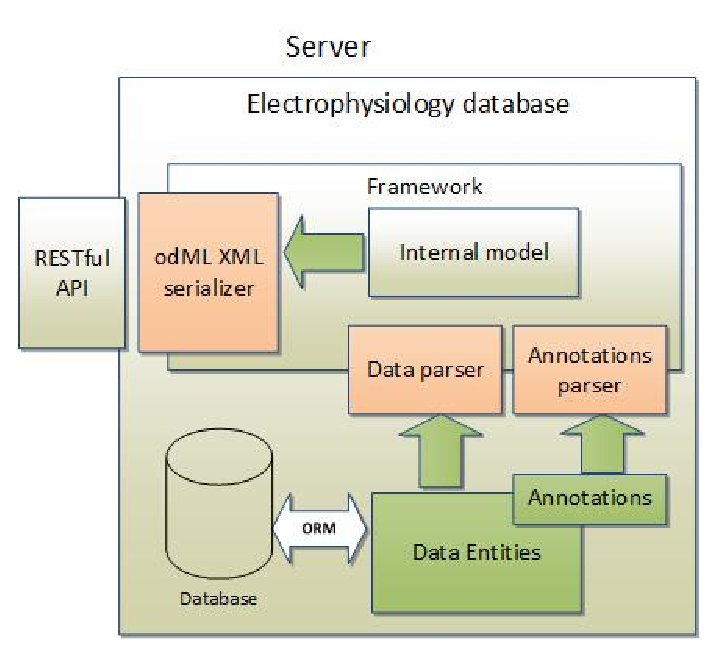
\includegraphics[width=9cm, height=8cm]{Framework}
\caption{\label{framework}Framework for Generating Templates and Data Transfer}

\end{figure}


\subsection{Mobile Client}

The mobile client is a framework implemented for the Android platform. A client block diagram is shown in Figure \ref{client}. A client input point is an odML deserializer that parses an input odML document into an internal model. The internal model can contain both data and templates. When the client requests a template, this template is transferred to a layout using a layout generator. When the client is requesting data for a specific layout, these data are processed by a data parser. Both layouts and data are stored in an embedded database (SQLLite). It enables users to work offline.

\begin{figure}
\centering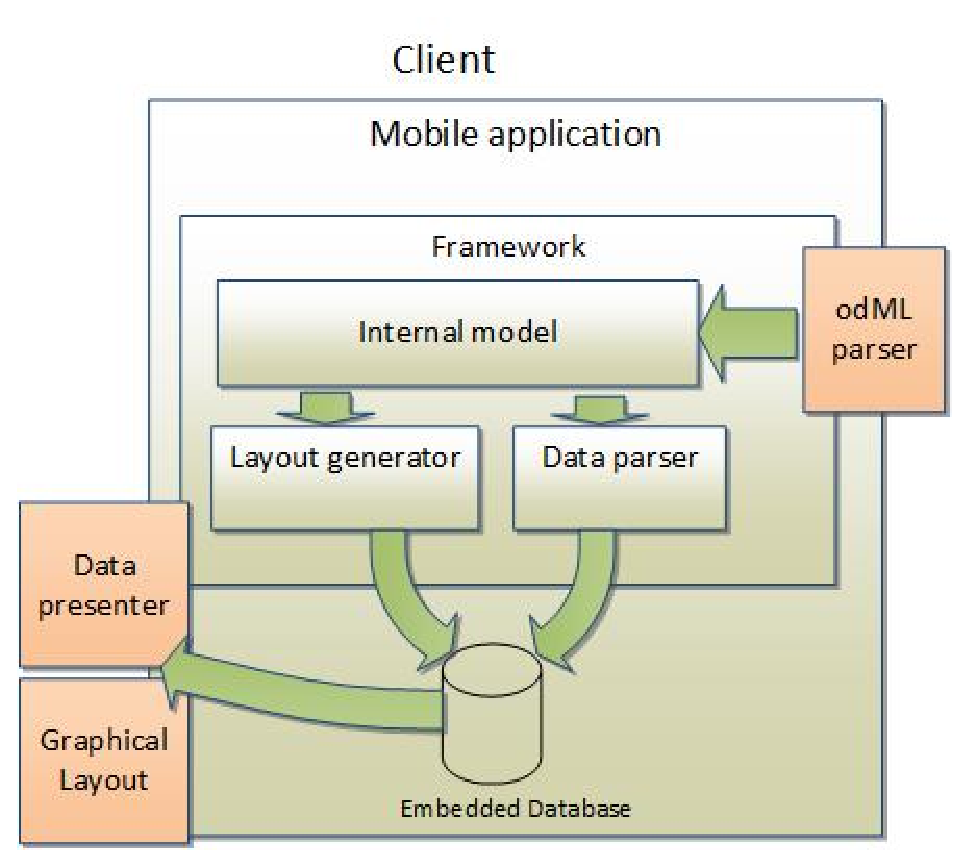
\includegraphics[width=9cm, height=6cm]{Client}
\caption{\label{client}Framework Implemented in the Mobile Client}

\end{figure}


\section{Use Case}

\subsection{Domain Specialization}

The main focus of the research group are methods and techniques of electroencephalography (EEG) and event-related-potentials (ERP). Experiments are conducted in a specialized laboratory equipped with highly specialized hardware and software. Except of this laboratory, we are equipped by a mobile laboratory that enables us to perform experiments outside. In addition we are cooperating in several INCF nodes including German, Belgian, USA or Japan nodes. Our equipment and a lot of discussion with our colleagues motivate us to design a test the solution described.

Experimental procedure follows several steps.  Experiments are performed according to defined scenario. Then data and metadata are collected. These data are analyzed and results are stored and published. The central point of this infrastructure is EEGBase \cite{DBLP:conf/biostec/JezekSBM13} that serves for storing and management of EEG/ERP experiments.

Although the system uses a web-based interface, a lot of experiments are conducted outside the laboratory when the common computer, or internet access are not available. The aim of this use case is to validate the integration of the presented framework and generation of templates according to data structure. Generation of templates is controlled by an Android phone. When the template is generated, new data can be collected and synchronized with EEGBase.

\subsection{EEGBase} \label{Portal}

EEGBase\footnote{https://eegdatabase.kiv.zcu.cz} is a mature web based system that enables registered users storing, sharing an managing EEG/ERP experiments. A user interface preview is shown in Figure \ref{portal}.

EEGBase provides a simple wizard that guides the user when uploading experiments. The user is instructed what metadata have to be filled in. The collected metadata respecting experience of our research partners with designing and performing experiments and experimental scenarios. The metadata follow ontology described in \cite{BMEI_jezek_moucek}.

The core structure contains the following semantic metadata groups:

\begin{itemize}
\item Scenario of experiment (name, length, description, ...)
\item Experimenters, tested people, experiment owner (given name, surname, contact, experiences, handicaps, ...)
\item Description of raw data (format, sampling frequency, ...)
\item Additional metadata in codebooks (weather, notes, electrode settings, artifact information, ...)
\end{itemize}


\begin{figure}
\centering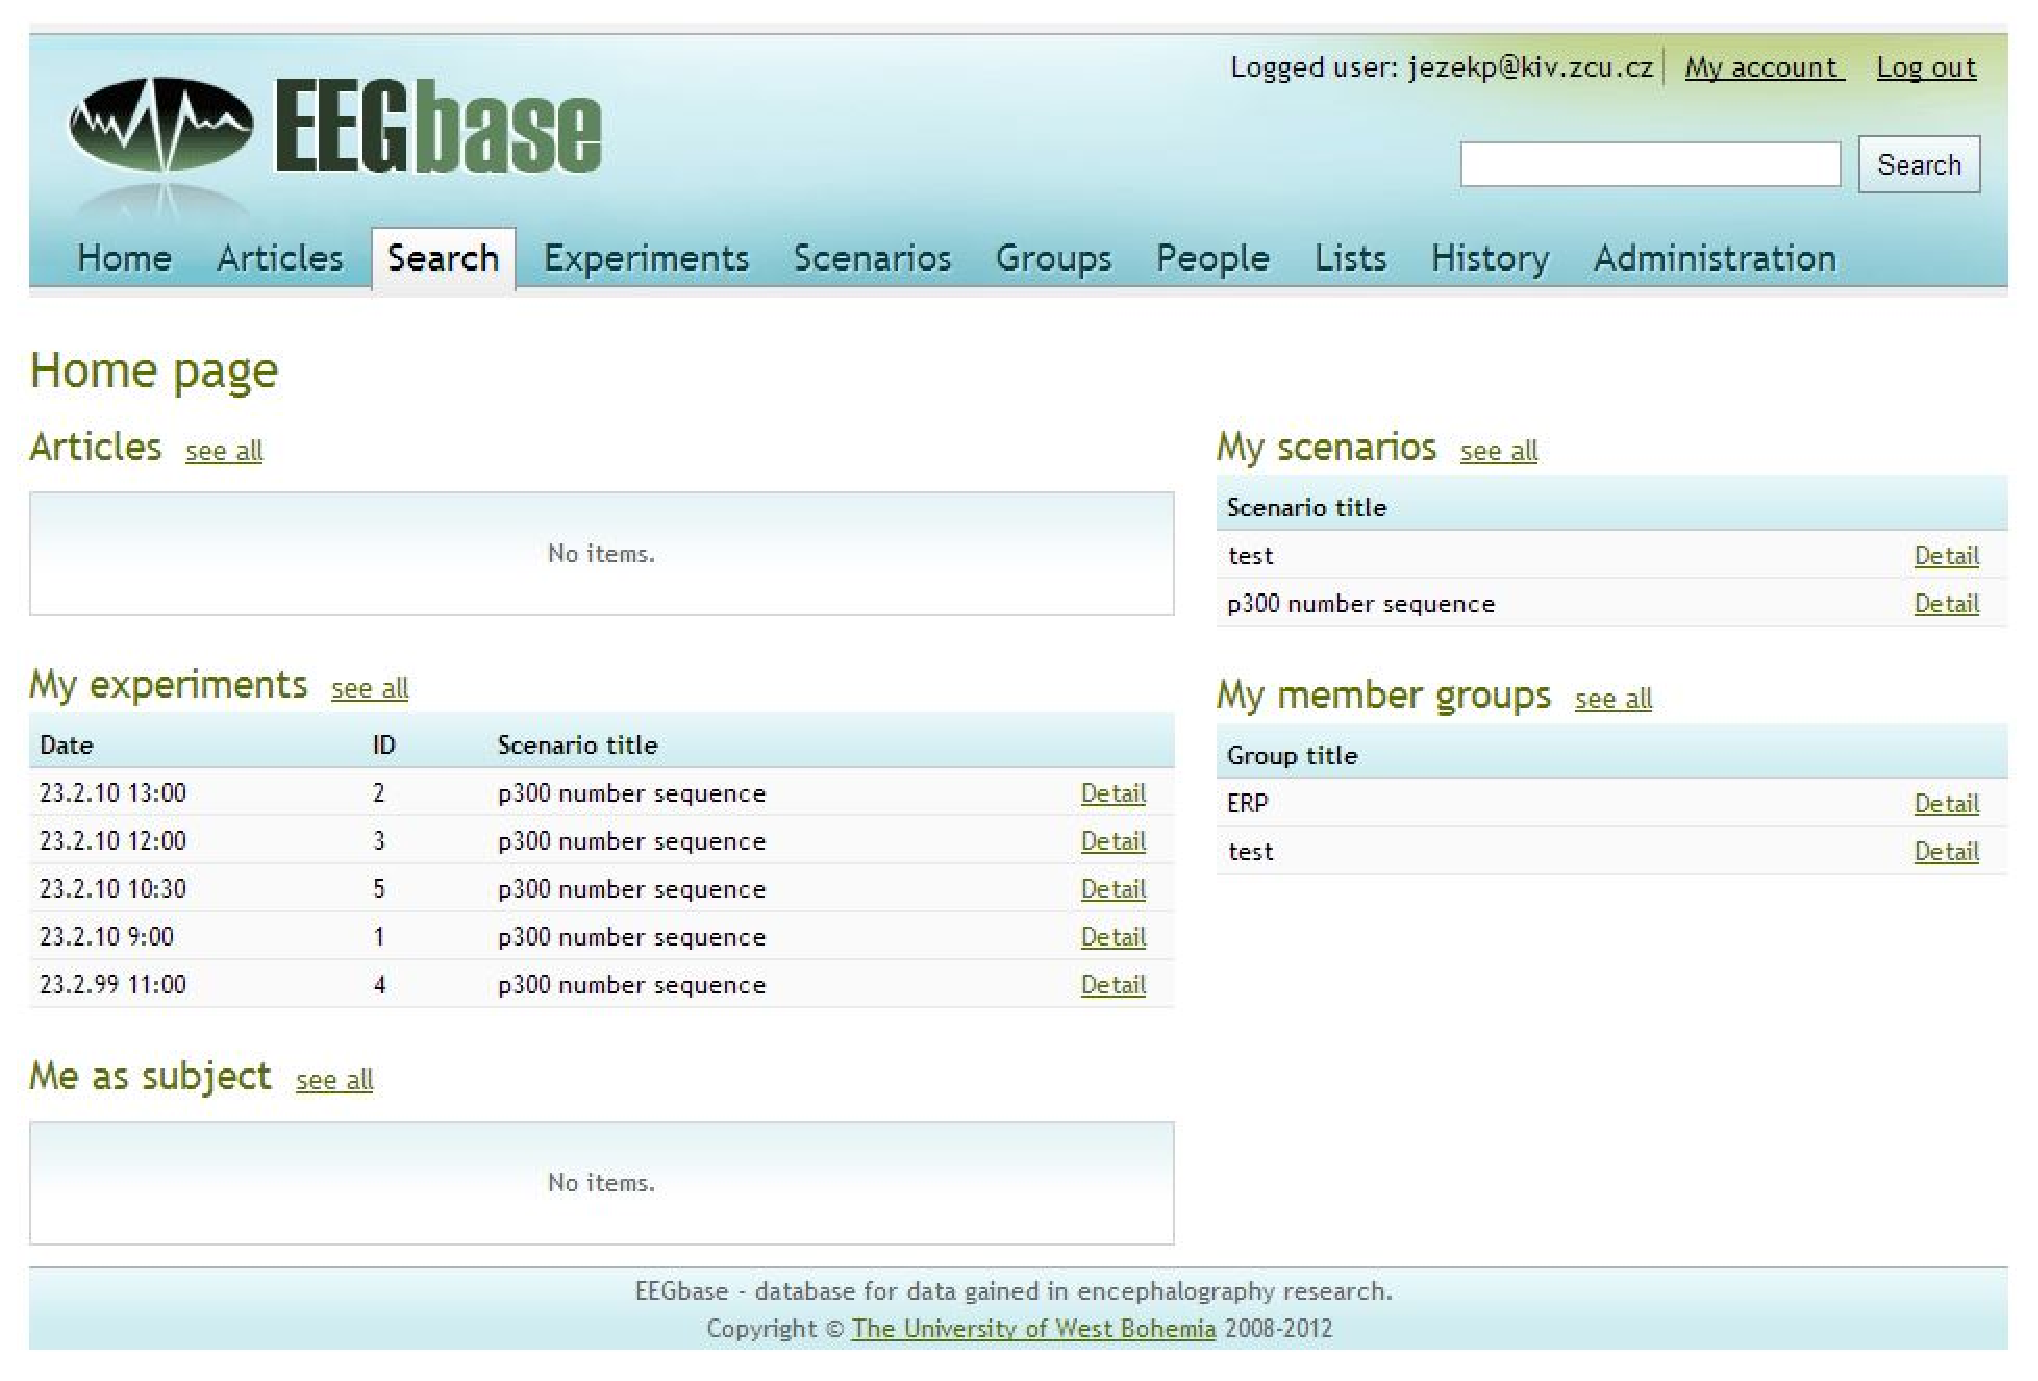
\includegraphics[width=8cm, height=5cm]{portal_preview}
\caption{\label{portal}EEGBase Preview}

\end{figure}

We prepared a simple proof-of-concept implementation based on a restricted set of metadata to demonstrate functionality of the framework. We selected the most important medata and annotate them by described annotations. Table \ref{entities_and_fields} shows selected entities with their annotated attributes.


\begin{table}
\begin{tabular}{|l|l|}
\hline
Entity & Annotated fields\\
\hline
Person     &
\begin{tabular}[c]{@{}l@{}}

@FormItem\\
	private String email;\\
	@FormItem(preview = PreviewLevel.MINOR)\\
	private String givenname;\\
	@FormItem(required = true, preview = PreviewLevel.MAJOR)\\
	private String surname;\\
	@FormItem\\
	private Timestamp dateOfBirth;\\
	@FormItem(required = true)\\
	@FormItemRestriction(values = {"M", "F"})\\
	private char gender;\\
	@FormItem(required = true)\\
	@FormItemRestriction(values = {"L", "R", "X"}, defaultValue = "X")\\
	private char laterality;\\
	private String phoneNumber;\\
	@FormItem\\
	private String note;

\end{tabular} \\
\hline
Scenario   &
\begin{tabular}[c]{@{}l@{}}


	@FormItem(required = true)\\
	private Person person;\\
	@FormItem(required = true)\\
	private ResearchGroup researchGroup;\\
	@FormItem(preview = PreviewLevel.MAJOR)\\
	private String title;\\
	@FormItem\\
    @FormItemRestriction(minLength =0)\\
	private int scenarioLength;\\
	@FormItem\\
	private boolean privateScenario;\\
	@FormItem\\
    @FormItemRestriction(maxLength = 255)\\
	private String description;\\
	@FormItem\\
	private String scenarioName;\\
	@FormItem\\
	private String mimetype;

\end{tabular} \\
\hline
Experiment &

\begin{tabular}[c]{@{}l@{}}

@FormItem(required = true)  \\
Weather weather;     \\
@FormItem(required = true, label = "Subject person")\\
private Person personBySubjectPersonId;\\
	@FormItem(required = true)\\
private Scenario scenario;\\
	@FormItem(required = true, label = "Owner")\\
private Person personByOwnerId;\\
	@FormItem(required = true)\\
private ResearchGroup researchGroup;\\
	@FormItem(required = true)\\
private Digitization digitization;\\
	@FormItem(required = true)\\
private SubjectGroup subjectGroup;\\
	@FormItem(required = true)\\
private Artifact artifact;\\
	@FormItem(required = true)\\
private ElectrodeConf electrodeConf;\\
	@FormItem(preview = PreviewLevel.MAJOR)\\
private Timestamp startTime;\\
	@FormItem\\
private Timestamp endTime;\\
	@FormItem\\
private int temperature;\\
	@FormItem\\
private boolean privateExperiment;\\
	@FormItem(preview = PreviewLevel.MINOR)\\
private String environmentNote;
\end{tabular}  \\

Stimulus   &
\begin{tabular}[c]{@{}l@{}}

@FormItemRestriction(maxLength = 255)\\
String description

\end{tabular} \\
\hline
DataFile   &

\begin{tabular}[c]{@{}l@{}}

@FormItemRestriction(maxLength = 255)\\
String description\\

\end{tabular}\\
\hline
\end{tabular}
\caption{Entities and their Annotated Fields}\label{entities_and_fields}
\end{table}

Since EEGBase implements RESTFull web services \cite{Richardson:2007:RWS:1406352}, control of the framework API by client requests is ensured. We implemented two methods; one for listing available templates and the second one for downloading a selected template\footnote{All API methods all described more in detail in a project wiki page: https://github.com/INCF/eeg-database/wiki/RESTful-API}.

\subsection{Mobile Client} \label{Mobile_Client}

The mobile client uses common design of Android applications. Main activities of the use-case study are shown in several screenshots in Figure \ref{fig:mob_app_prev}. Because the client is intended to work with various electrophysiological databases, it enables creating separate workspaces where each workspace works with different user credentials. In Figure \ref{fig:mob_app_preva} the user creates a new workspace. Users credentials are optional because the client can work as a stand alone system as well. In Figure \ref{fig:mob_app_prevb} available layouts are listed; the user can download them. Finally, in Figure \ref{fig:mob_app_prevc} the user can download data from the server or add new data as shown in Figure \ref{fig:mob_app_prevd}.

By following the described steps we created one workspace connected to EEGBase (see Figure\ref{fig:mob_app_preva}) and downloaded available layouts (Person, Scenario, Experiment and DataFile as listed in Figure \ref{fig:mob_app_prevb}). When the layouts were downloaded experiments from the server were listed (see Figure \ref{fig:mob_app_prevc}). Finally, we add several new experiments using form listed in Figure \ref{fig:mob_app_prevd}. These experiments were stored on the server.

\begin{figure*}
% Use the relevant command to insert your figure file.
% For example, with the graphicx package use
\begin{tabular}{c}
\subfloat[The user can create a new workspace]{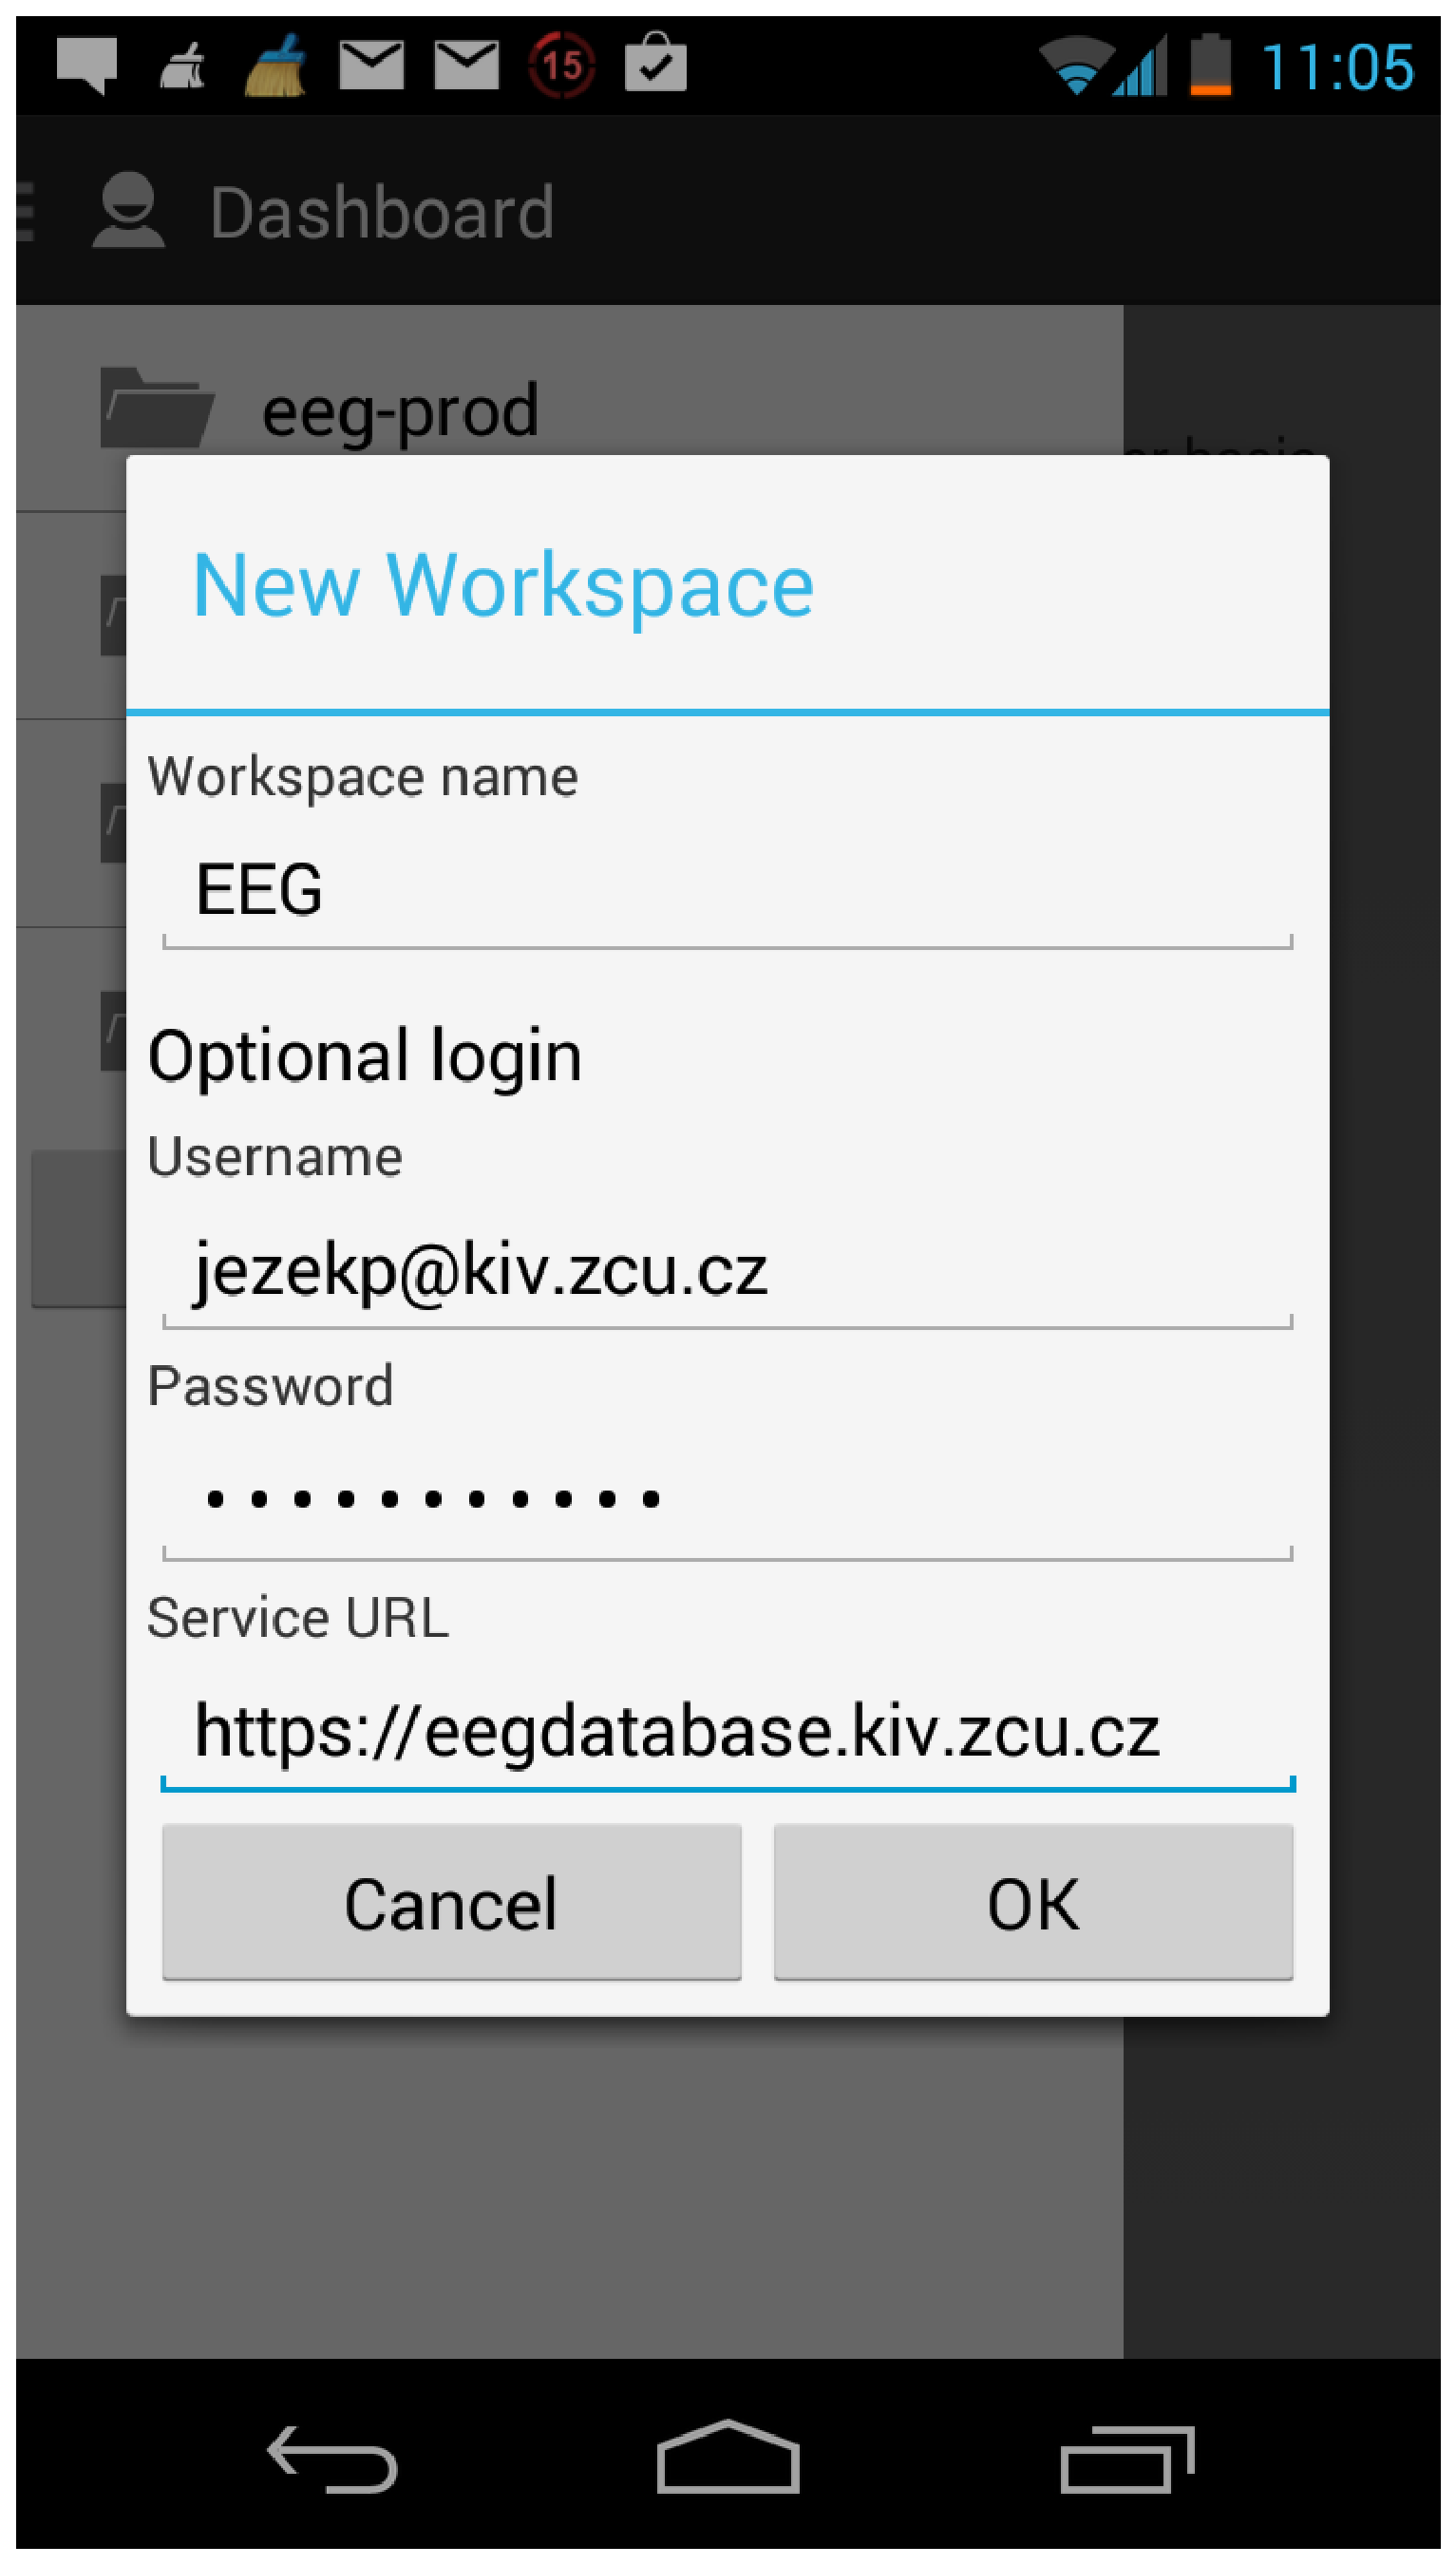
\includegraphics[width = 4cm, height=7cm]{2014-07-02090600}\label{fig:mob_app_preva}}
\hspace{10pt}\subfloat[Then select available layout]{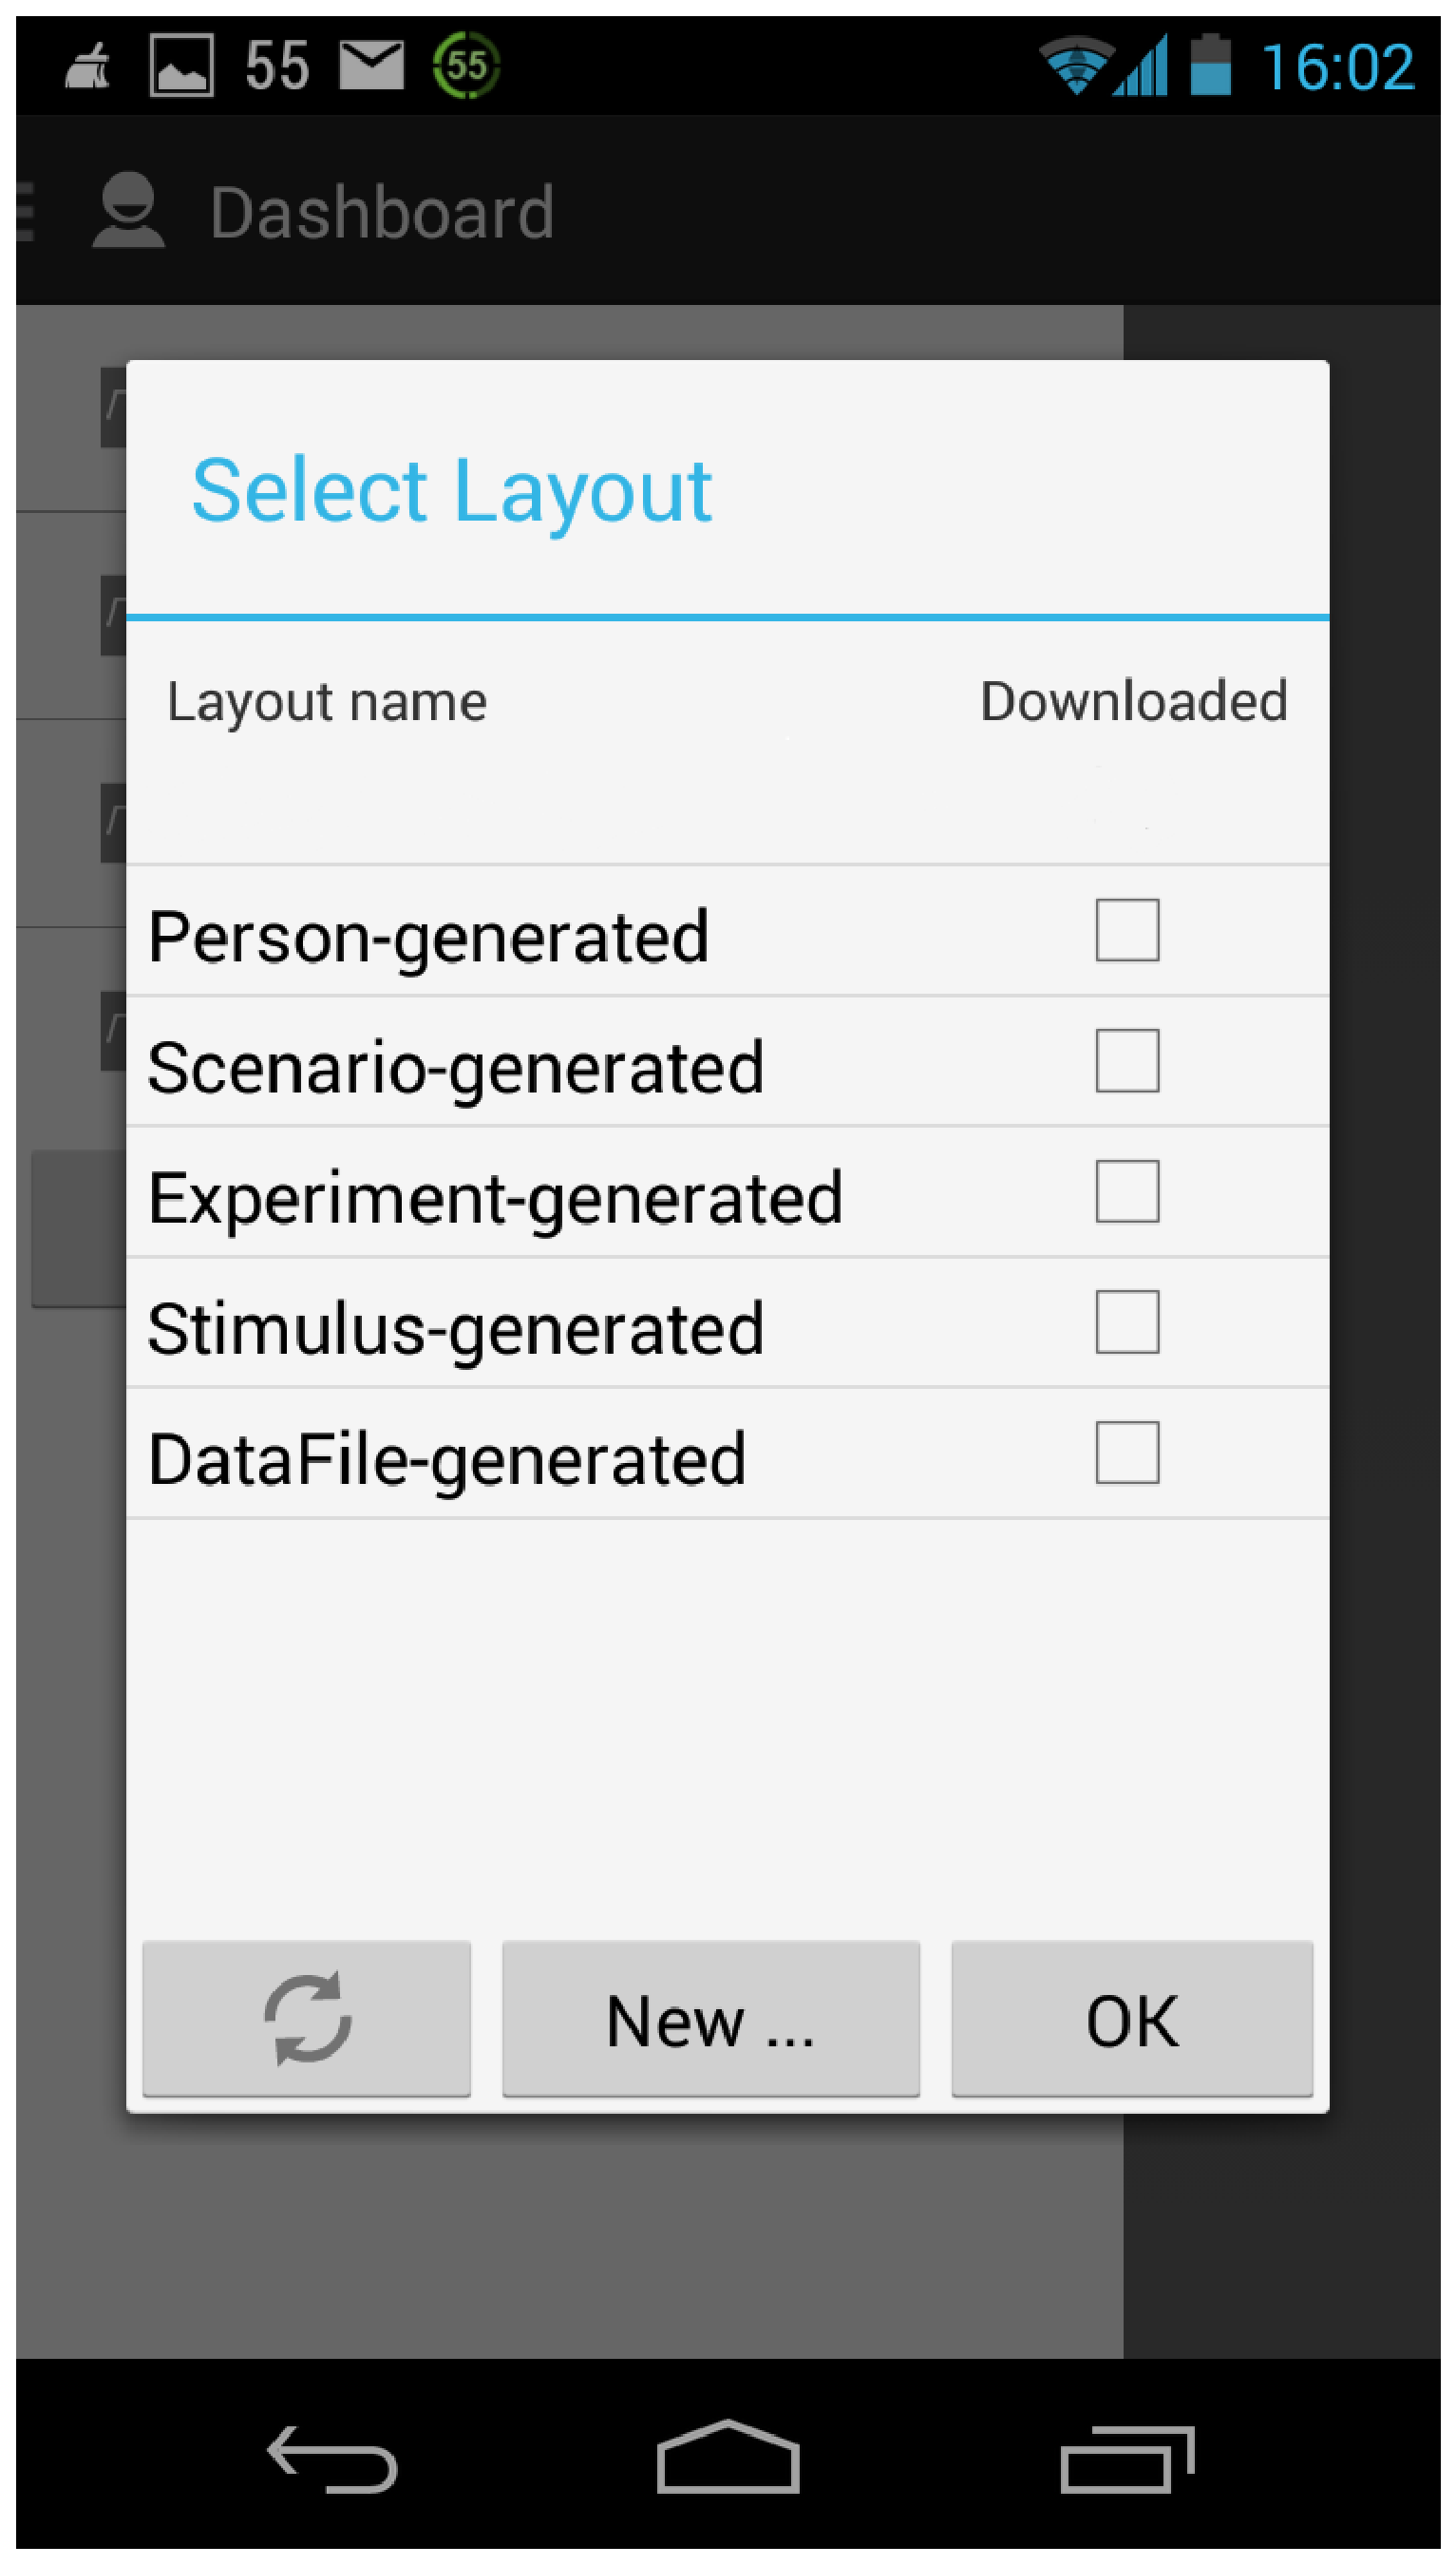
\includegraphics[width = 4cm, height=7cm]{2014-06-26140214}\label{fig:mob_app_prevb}}
\hspace{10pt}\subfloat[Finally list data]{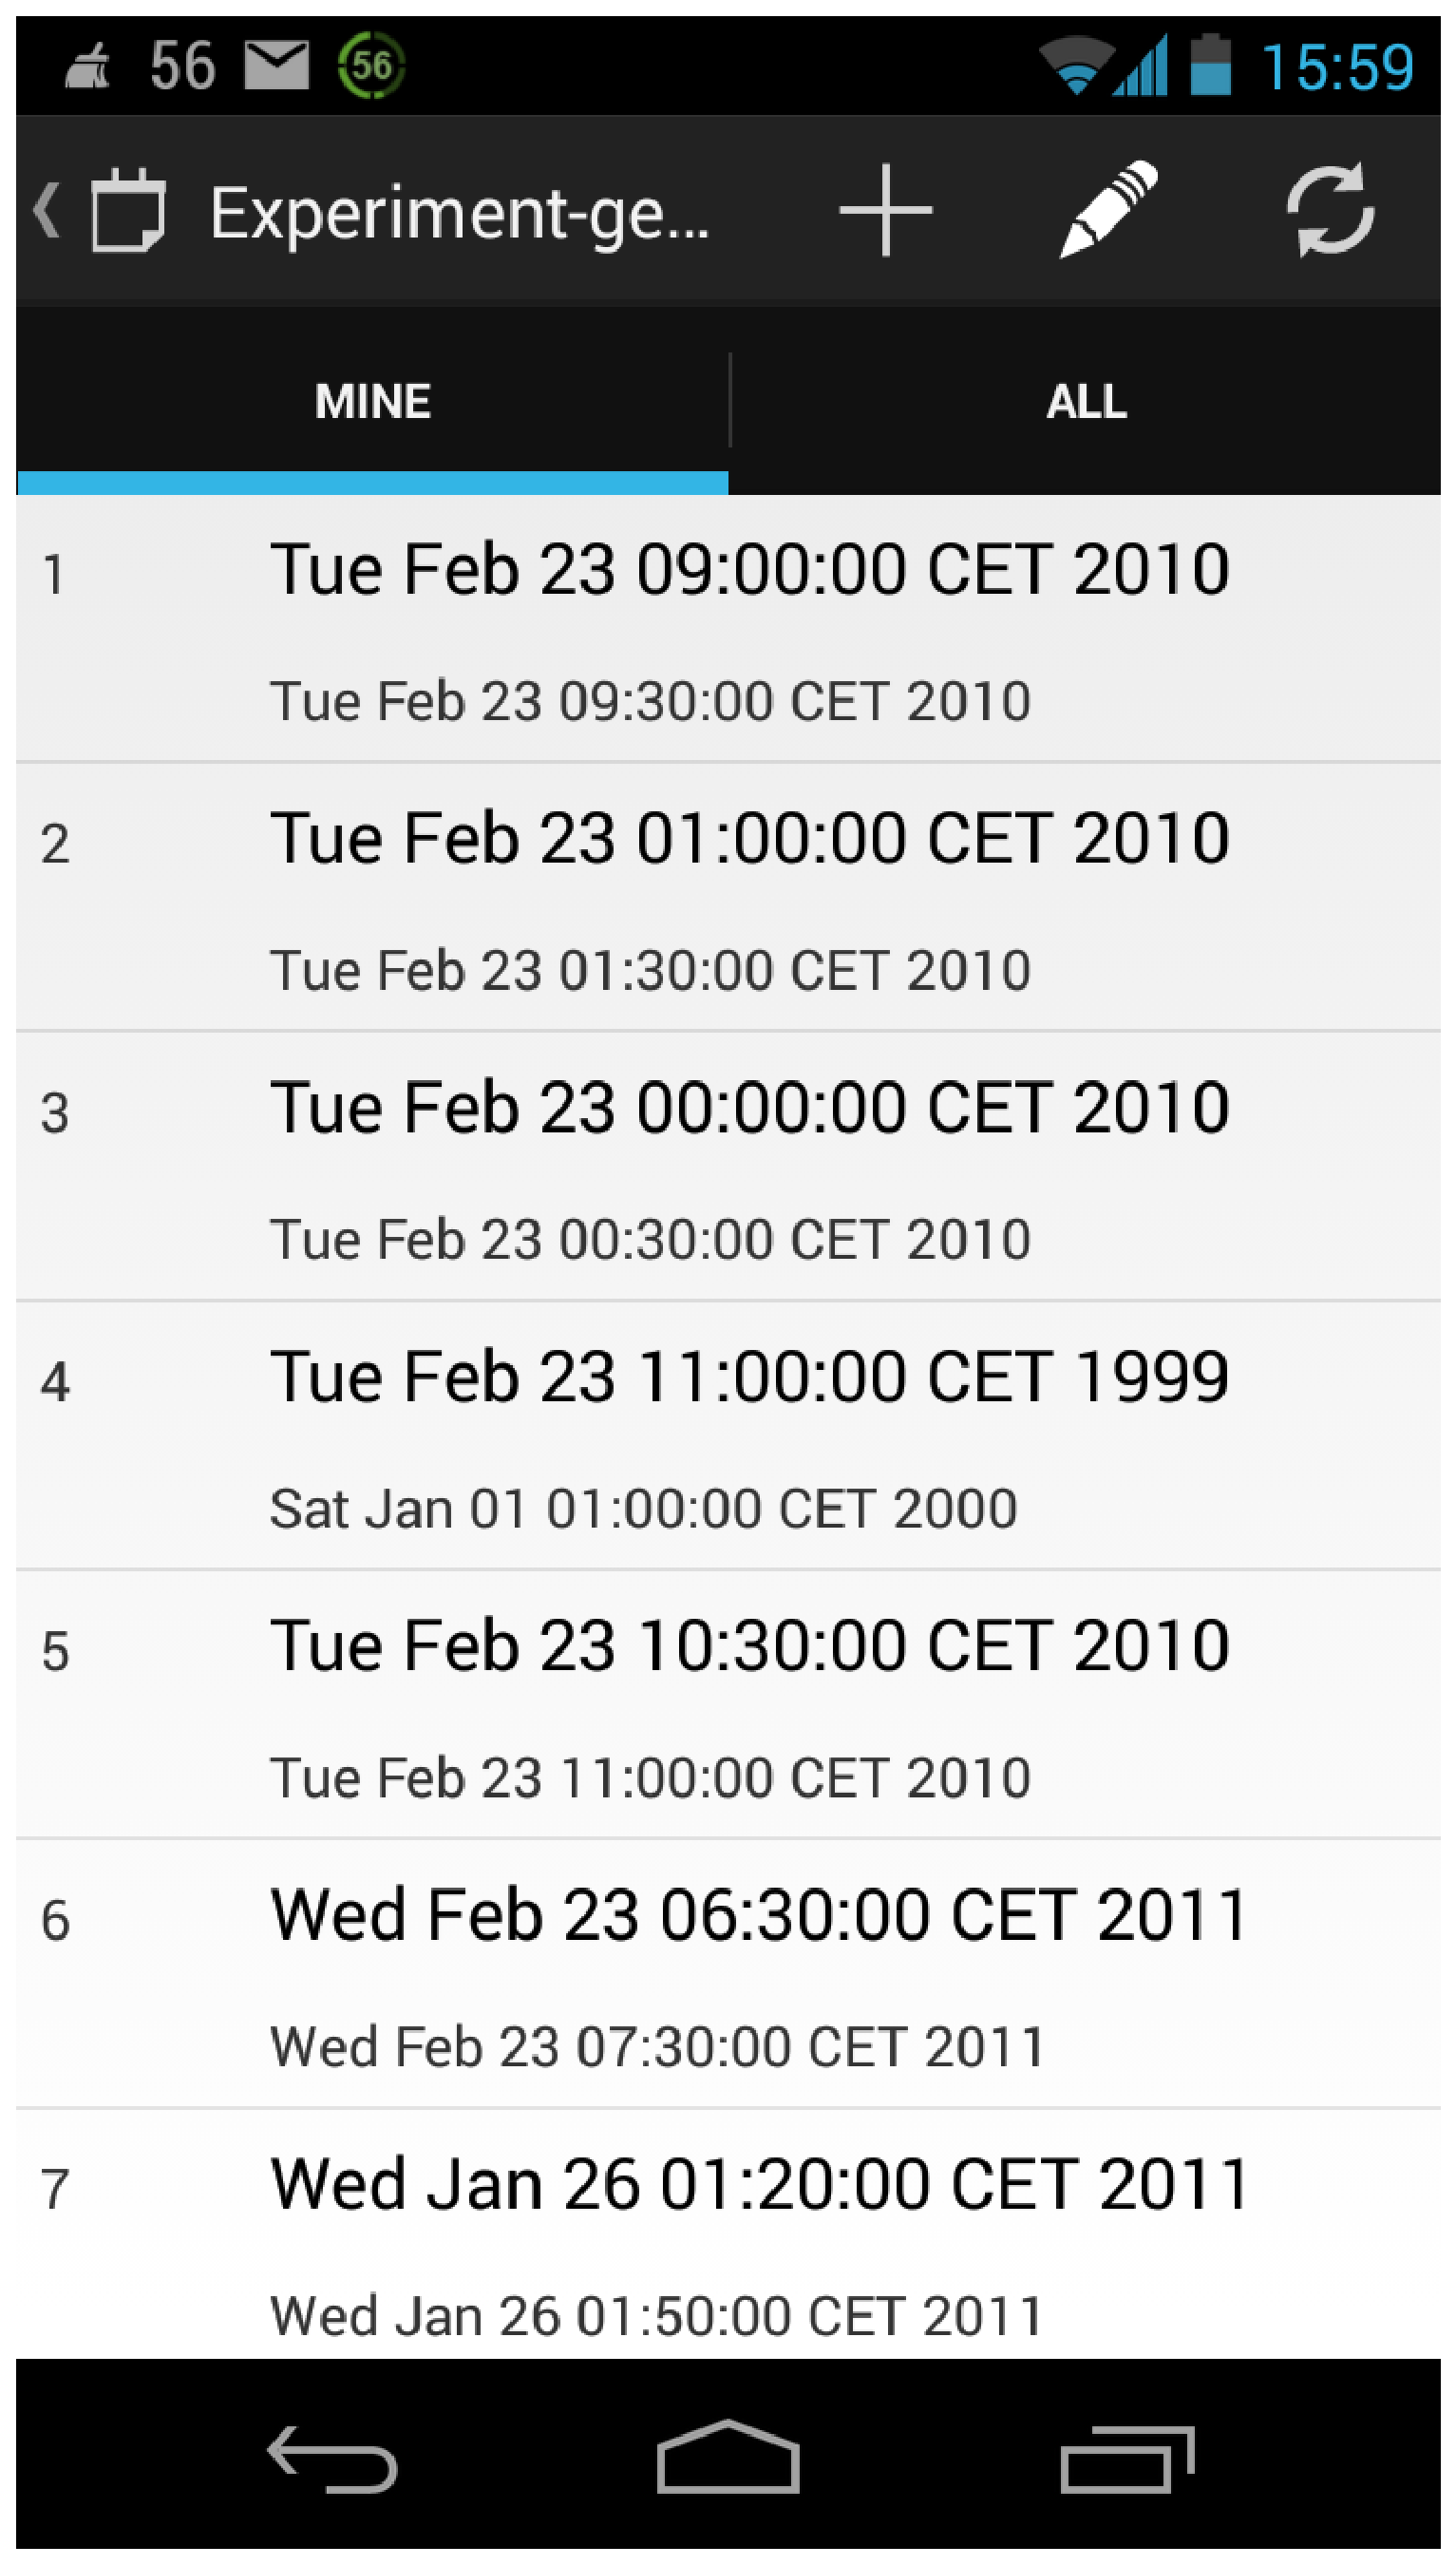
\includegraphics[width = 4cm, height=7cm]{2014-06-26135912}\label{fig:mob_app_prevc}}
\hspace{10pt}\subfloat[He/she can add a new item when clicks to a + button]{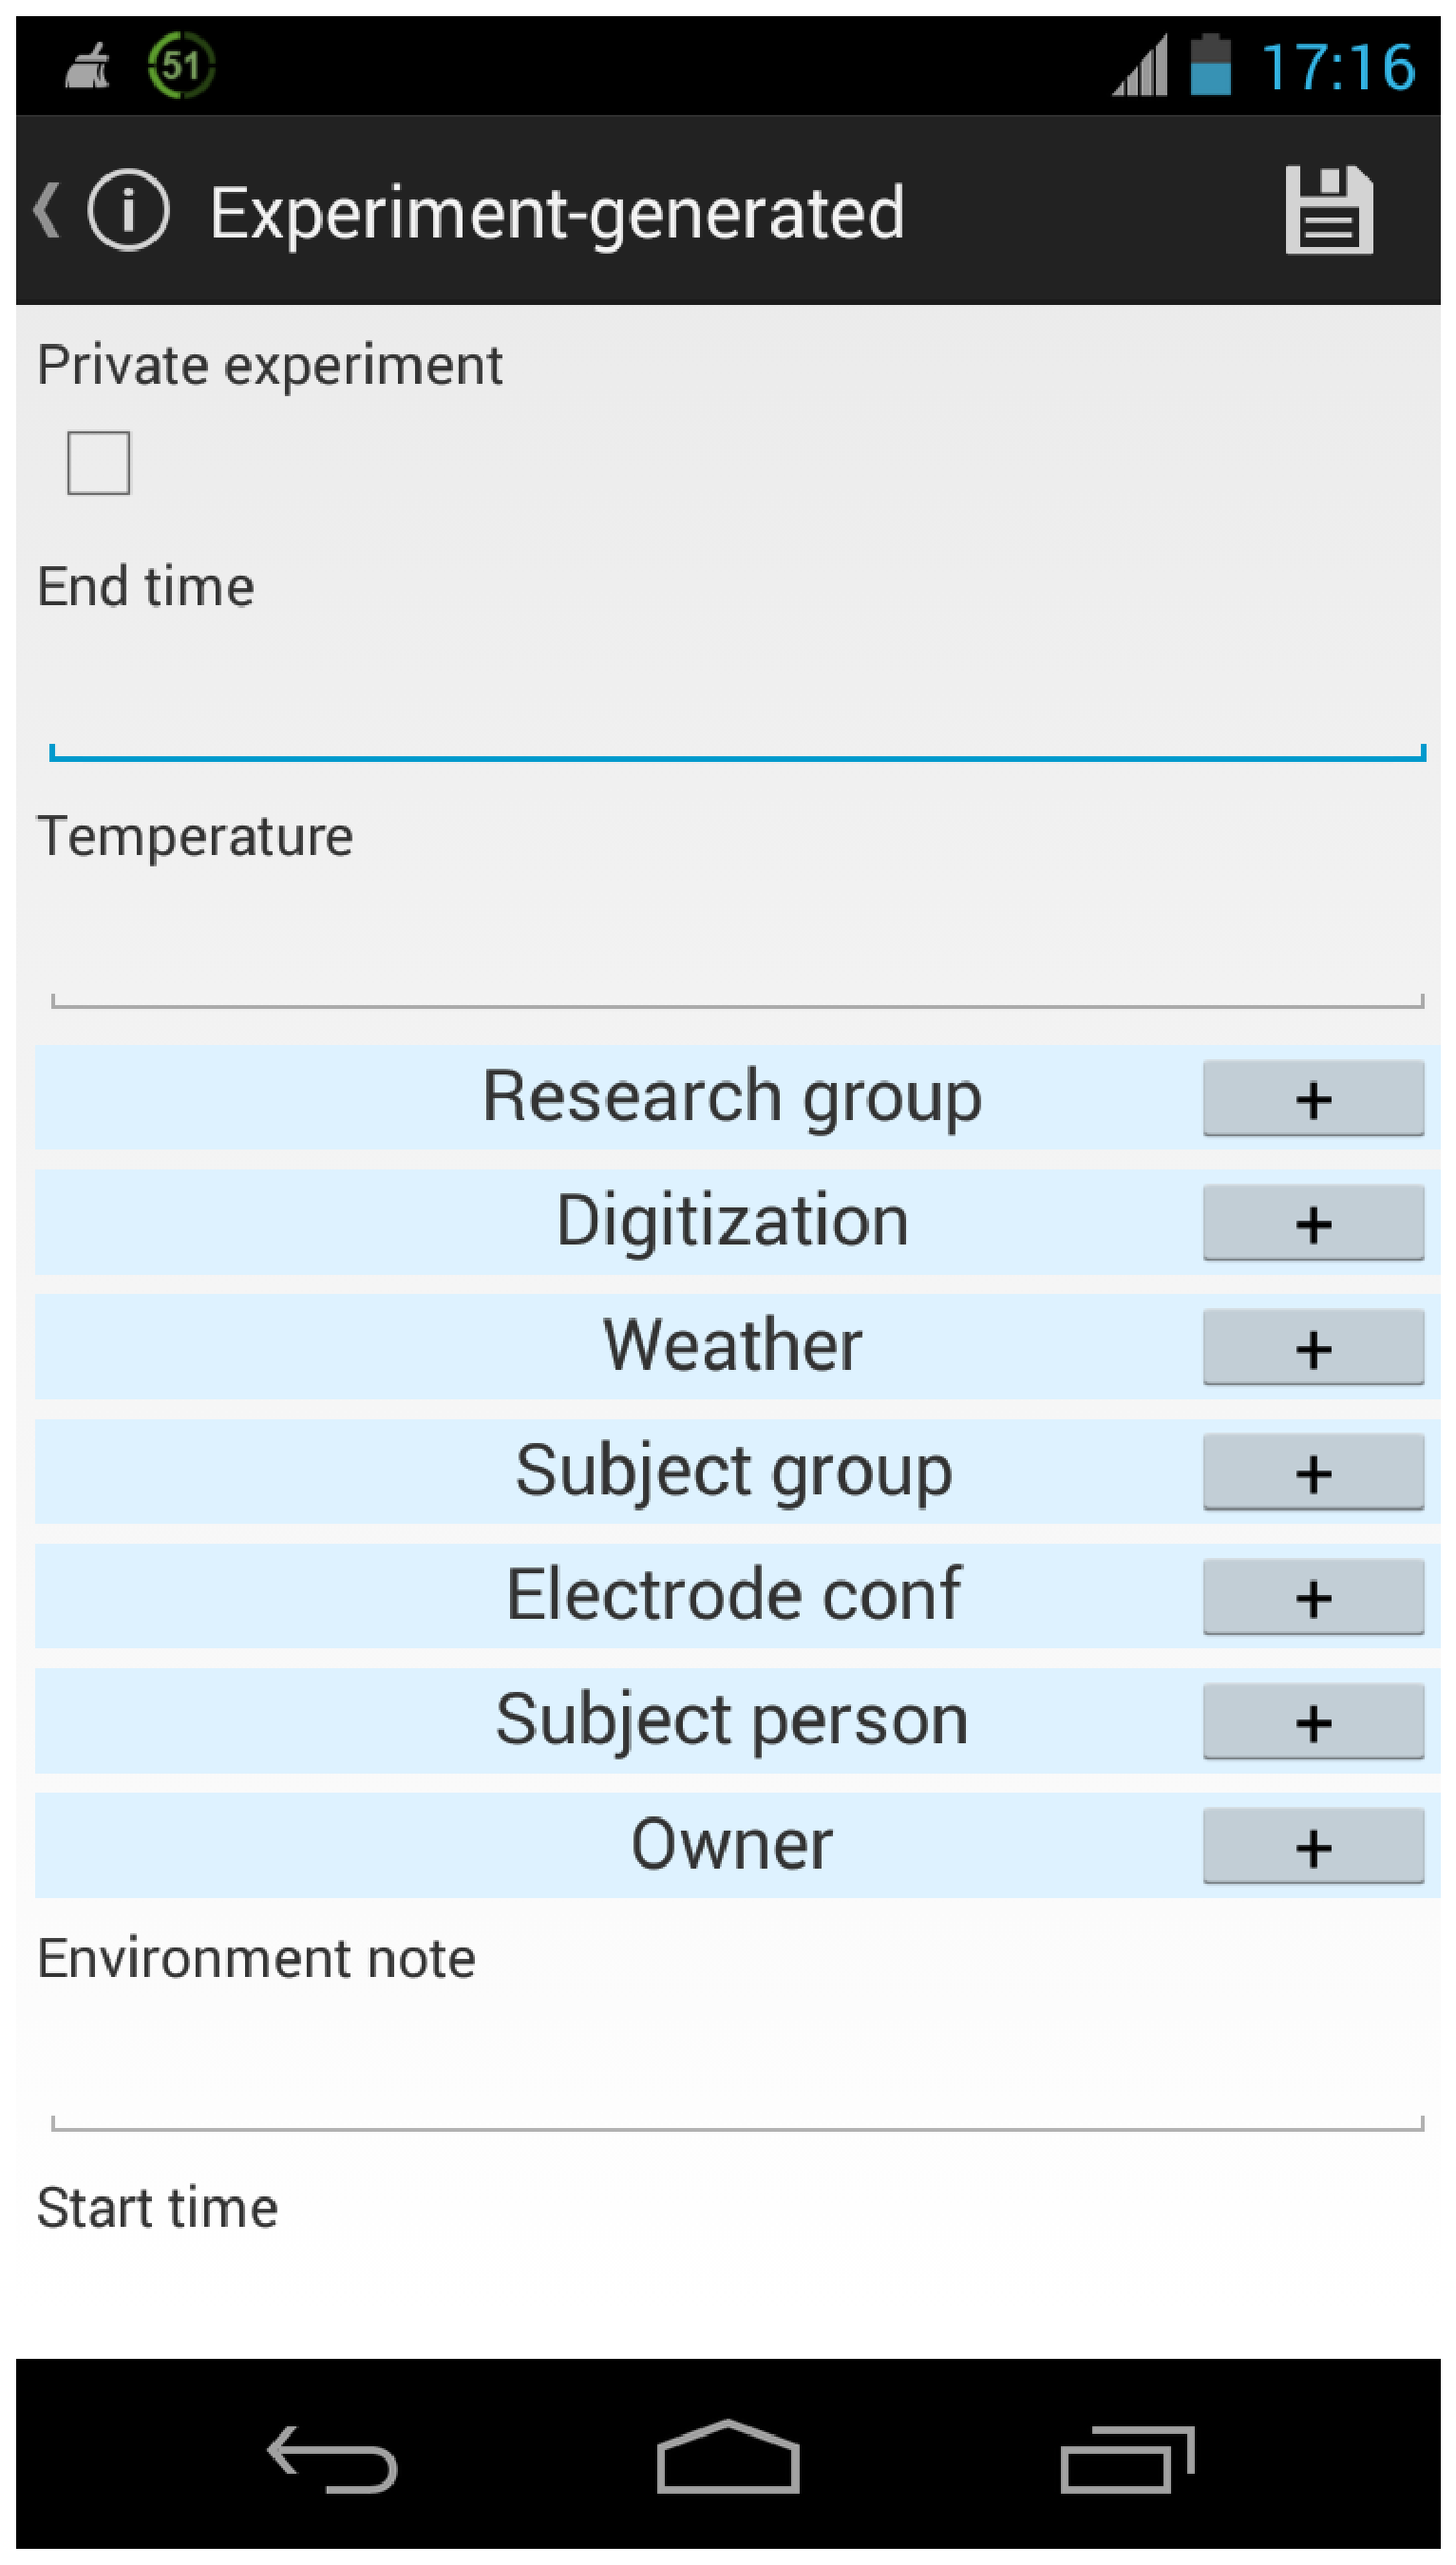
\includegraphics[width = 4cm, height=7cm]{2014-07-03151609}\label{fig:mob_app_prevd}}
\end{tabular}
% figure caption is below the figure
\caption{Mobile Application Use Case Preview}
\label{fig:mob_app_prev}
\end{figure*}



% An example of a floating figure using the graphicx package.
% Note that \label must occur AFTER (or within) \caption.
% For figures, \caption should occur after the \includegraphics.
% Note that IEEEtran v1.7 and later has special internal code that
% is designed to preserve the operation of \label within \caption
% even when the captionsoff option is in effect. However, because
% of issues like this, it may be the safest practice to put all your
% \label just after \caption rather than within \caption{}.
%
% Reminder: the "draftcls" or "draftclsnofoot", not "draft", class
% option should be used if it is desired that the figures are to be
% displayed while in draft mode.
%
%\begin{figure}[!t]
%\centering
%\includegraphics[width=2.5in]{myfigure}
% where an .eps filename suffix will be assumed under latex,
% and a .pdf suffix will be assumed for pdflatex; or what has been declared
% via \DeclareGraphicsExtensions.
%\caption{Simulation Results}
%\label{fig_sim}
%\end{figure}

% Note that IEEE typically puts floats only at the top, even when this
% results in a large percentage of a column being occupied by floats.


% An example of a double column floating figure using two subfigures.
% (The subfig.sty package must be loaded for this to work.)
% The subfigure \label commands are set within each subfloat command, the
% \label for the overall figure must come after \caption.
% \hfil must be used as a separator to get equal spacing.
% The subfigure.sty package works much the same way, except \subfigure is
% used instead of \subfloat.
%
%\begin{figure*}[!t]
%\centerline{\subfloat[Case I]\includegraphics[width=2.5in]{subfigcase1}%
%\label{fig_first_case}}
%\hfil
%\subfloat[Case II]{\includegraphics[width=2.5in]{subfigcase2}%
%\label{fig_second_case}}}
%\caption{Simulation results}
%\label{fig_sim}
%\end{figure*}
%
% Note that often IEEE papers with subfigures do not employ subfigure
% captions (using the optional argument to \subfloat), but instead will
% reference/describe all of them (a), (b), etc., within the main caption.


% An example of a floating table. Note that, for IEEE style tables, the
% \caption command should come BEFORE the table. Table text will default to
% \footnotesize as IEEE normally uses this smaller font for tables.
% The \label must come after \caption as always.
%
%\begin{table}[!t]
%% increase table row spacing, adjust to taste
%\renewcommand{\arraystretch}{1.3}
% if using array.sty, it might be a good idea to tweak the value of
% \extrarowheight as needed to properly center the text within the cells
%\caption{An Example of a Table}
%\label{table_example}
%\centering
%% Some packages, such as MDW tools, offer better commands for making tables
%% than the plain LaTeX2e tabular which is used here.
%\begin{tabular}{|c||c|}
%\hline
%One & Two\\
%\hline
%Three & Four\\
%\hline
%\end{tabular}
%\end{table}


% Note that IEEE does not put floats in the very first column - or typically
% anywhere on the first page for that matter. Also, in-text middle ("here")
% positioning is not used. Most IEEE journals/conferences use top floats
% exclusively. Note that, LaTeX2e, unlike IEEE journals/conferences, places
% footnotes above bottom floats. This can be corrected via the \fnbelowfloat
% command of the stfloats package.

\section{Future Work}

The proposed solution works satisfactorily and the presented use-case study validates its functionality on real data. However, the presented pilot implementation has several gaps that are planned to be overcome. Probably the most important, is its focus on electrophysiology databases storing data in relational databases. Because electrophysiological data are heterogeneous, the usage of NoSQL databases seems to be more practical. Our test proves \cite{Jezek2014422} that a shift from a relational database to a NoSQL one brings a lot of benefits handling metadata. The very first next step is to propose a suitable mapping of heterogeneous metadata stored in a NoSQL database to a suitable data template. The next improvement includes an extension of the mobile client to other platforms (iPhone, Windows Phone)\footnote{several frameworks as http://phonegap.com/ enables development of platform independent mobile applications} and extension of the server part of the framework not to work only with Java-based servers.

\section{Conclusion}

Experiments in electrophysiology domain produce a lot of collections of semi-structured data and metadata. To organize these metadata, various data formats implemented in electrophysiological databases have been introduced. Data in these databases are accessed from laboratory computers using fixed user interfaces. Therefore these databases are unreachable where a common computer is not available. With expansion of mobile devices users would like to manage data using their smart phones. Because the dual development of user interfaces for both common computers and mobile devices increases demands to developers and reduces users experience with these systems, we proposed an annotation framework that enables to generate graphical layouts for mobile devices automatically. This framework enables users to map a data layer of an electrophysiological database and create the template representing the data structure. This template is serialized to an odML document and transferred to the client system. The client system parses this template and generates a graphical layout displayed in the device. In addition, when the layout is prepared, the experimental data can be synchronized with the server.


% conference papers do not normally have an appendix


% use section* for acknowledgement
\section*{Acknowledgment}


This work was supported by the European Regional Development Fund (ERDF), Project "NTIS - New Technologies for Information Society", European Centre of Excellence, CZ.1.05/1.1.00/02.0090 and by the UWB grant SGS-2013-039 Methods and Applications of Bio- and Medical Informatics.




% trigger a \newpage just before the given reference
% number - used to balance the columns on the last page
% adjust value as needed - may need to be readjusted if
% the document is modified later
%\IEEEtriggeratref{8}
% The "triggered" command can be changed if desired:
%\IEEEtriggercmd{\enlargethispage{-5in}}

% references section�

% can use a bibliography generated by BibTeX as a .bbl file
% BibTeX documentation can be easily obtained at:
% http://www.ctan.org/tex-archive/biblio/bibtex/contrib/doc/
% The IEEEtran BibTeX style support page is at:
% http://www.michaelshell.org/tex/ieeetran/bibtex/
\bibliographystyle{IEEEtran}
% argument is your BibTeX string definitions and bibliography database(s)
\bibliography{bibliography,neuroportals,frontiers}
%
% <OR> manually copy in the resultant .bbl file
% set second argument of \begin to the number of references
% (used to reserve space for the reference number labels box)



% that's all folks
\end{document}


